\documentclass[a4paper,11pt]{article}
\input{/home/tof/Documents/Cozy/latex-include/preambule_lua.tex}
\newcommand{\showprof}{show them}  % comment this line if you don't want to see todo environment
\fancyhead[L]{Arbre binaire - Roland Garros}
\newdate{madate}{10}{09}{2020}
%\fancyhead[R]{\displaydate{madate}} %\today
%\fancyhead[R]{Seconde - SNT}
%\fancyhead[R]{Première - NSI}
\fancyhead[R]{Terminale - NSI}
\fancyfoot[L]{~\\Christophe Viroulaud}
\AtEndDocument{\label{lastpage}}
\fancyfoot[C]{\textbf{Page \thepage/\pageref{lastpage}}}
\fancyfoot[R]{\includegraphics[width=2cm,align=t]{/home/tof/Documents/Cozy/latex-include/cc.png}}
\usepackage{tikz}

\begin{document}
\begin{Form}
\section{Problématique}
Le comité du \emph{grand chelem de Roland Garros} réorganise la gestion numérique du tableau du tournoi afin de pouvoir fournir des statistiques sur le parcours de chaque joueur dans la quinzaine.
\begin{center}
\centering
\includegraphics[width=5cm]{ressources/rg.jpg}
\captionof{figure}{Tableau Dames}
\label{rg}
\end{center}

\begin{center}
\shadowbox{\parbox{15cm}{\centering Quelle structure de données peut-on utiliser pour représenter le tableau du tournoi?}}
\end{center}
\section{Arbre binaire}
\subsection{Définition}
Un \emph{arbre binaire} est un cas particulier des structures arborescentes.
\begin{aretenir}[]
Un \textbf{arbre binaire} est une structure arborescente où chaque nœud possède \textbf{au plus} deux fils. L'ordre des nœuds-fils est pris en compte: on parle alors de fils \emph{gauche} et fils \emph{droit}.
\end{aretenir}
\begin{commentprof}
Le vocabulaire défini précédemment s'applique donc pour ce cas de figure.\\
sous-arbre gauche et droit\\
nœud interne = qui a au moins 1 enfant (pas les feuilles donc)
\end{commentprof}
La représentation d'un nœud n'est pas généralisée dans la littérature (figure \ref{noeud}).
\begin{center}
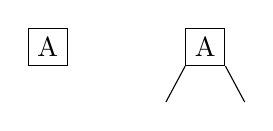
\begin{tikzpicture}
\node[draw] (A) at (0,0) {A};
\node[draw] (B) at (2,0) {A};

\draw (B.south west) -- (1.5,-0.7);
\draw (B.south east) -- (2.5,-0.7);
\end{tikzpicture}
\captionof{figure}{Représentations d'un nœud}
\label{noeud}
\end{center}
\begin{center}
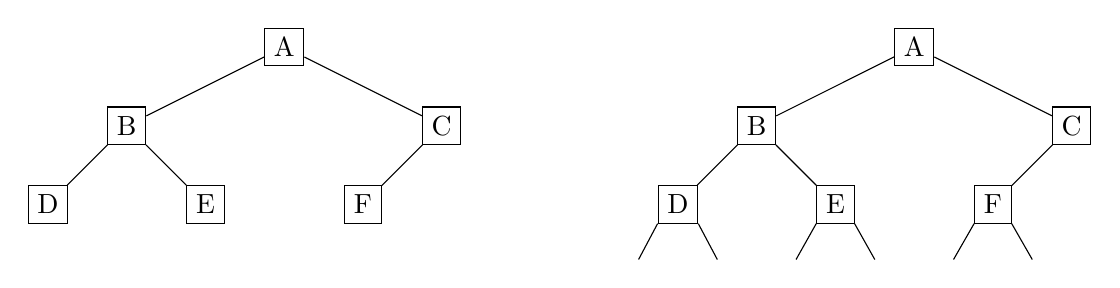
\begin{tikzpicture}
\node[draw] (A) at (-3,0) {A};
\node[draw] (B) at (-5,-1) {B};
\node[draw] (C) at (-1,-1) {C};
\node[draw] (D) at (-6,-2) {D};
\node[draw] (E) at (-4,-2) {E};
\node[draw] (F) at (-2,-2) {F};

\draw (A) -- (B);
\draw (A) -- (C);
\draw (B) -- (D);
\draw (B) -- (E);
\draw (C) -- (F);

\node[draw] (A1) at (5,0) {A};
\node[draw] (B1) at (3,-1) {B};
\node[draw] (C1) at (7,-1) {C};
\node[draw] (D1) at (2,-2) {D};
\node[draw] (E1) at (4,-2) {E};
\node[draw] (F1) at (6,-2) {F};

\draw (A1) -- (B1);
\draw (A1) -- (C1);
\draw (B1) -- (D1);
\draw (B1) -- (E1);
\draw (C1) -- (F1);
\draw (D1.south west) -- (1.5,-2.7);
\draw (D1.south east) -- (2.5,-2.7);
\draw (E1.south west) -- (3.5,-2.7);
\draw (E1.south east) -- (4.5,-2.7);
\draw (F1.south west) -- (5.5,-2.7);
\draw (F1.south east) -- (6.5,-2.7);
\end{tikzpicture}
\captionof{figure}{Représentations d'un arbre binaire}
\label{arbre}
\end{center}
Un arbre binaire est:
\begin{itemize}
\item \textbf{équilibré} si pour chaque nœud interne, les \emph{sous-arbres gauche et droite} ont une hauteur qui diffère au plus de 1,
\item \textbf{complet} si tous les niveaux sont remplis sauf éventuellement le dernier; les feuilles sont alors \emph{tassées à gauche},
\item \textbf{parfait} si tous les niveaux sont remplis.
\end{itemize}

\subsection{Hauteur}
La \textbf{taille} représente le nombre de nœuds qui composent l'arbre. La \textbf{hauteur (ou profondeur)} est la longueur du plus grand chemin entre la racine et une feuille.
\begin{aretenir}[]
Dans un arbre binaire, la taille \emph{N} et la hauteur \emph{h} sont liées par les inégalités:
\begin{center}
$h+1 \leqslant N \leqslant 2^{h+1}-1$
\end{center}
\end{aretenir}
\begin{commentprof}
hauteur arbre vide = -1
\end{commentprof}
\begin{aretenir}[Remarque]
Si la définition de la hauteur est définie comme le nombre maximum de nœuds entre la racine et une feuille, cette propriété s'écrit:
\begin{center}
$h \leqslant N \leqslant 2^{h}-1$
\end{center}
\end{aretenir}

\section{Représentation d'un arbre binaire}
\end{Form}
\end{document}